\documentclass[tikz,border=10pt]{standalone}
\usetikzlibrary{patterns}

\begin{document}
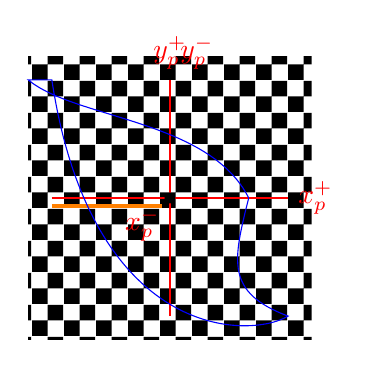
\begin{tikzpicture}
    % Define the coordinates for the center point p
    \coordinate (p) at (0,0);
    
    % Draw the checkerboard pattern fill for the surrounding area
    \path[pattern=checkerboard] (-1.8,-1.8) rectangle (1.8,1.8);
    
    % Draw the red lines for x_p^- , x_p^+ , y_p^- , and y_p^+
    \draw[red, thick] (-1.5,0) -- (1.5,0) node[right] {$x_p^+$};
    \draw[red, thick] (0,-1.5) -- (0,1.5) node[above] {$y_p^+$};
    \draw[red, thick] (-1.5,0) -- (0,0) node[below left] {$x_p^-$} ;
    \draw[red, thick] (0,0) -- (0,1.5) node[above right] {$y_p^-$};
    
    % Mark the central point p
    \fill (p) circle (2pt);
    
    % Highlight a specific segment with a thick orange line
    \draw[orange, very thick] (-1.5,-0.1) -- (-0.1,-0.1);
    
    % Draw the irregular outer boundary
    \draw[blue] (-1.8,1.5) .. controls (-1.2,1) and (0.5,1) .. (1,0) .. controls (0.8,-0.8) and (0.7,-1.2) .. (1.5,-1.5)
        .. controls (1,-1.8) and (-1,-1.8) .. (-1.5,1.5) -- cycle;
\end{tikzpicture}
\end{document}